\section{ESCHER Design and Workflow}
\label{sec:arch}


% Express in three variables - Resource time and spatial.
A scheduling policy is defined by a set of temporal and spatial dependencies between tasks and nodes. We call these dependencies \emph{scheduling constraints}. 
%More precisely, scheduling constraints specify "when" and "where" (i.e., on which node) should a set of tasks be executed. Given the set of all tasks $W$, a scheduler must provide a schedule in the form of a one-to-many mapping of $S_t$ from $W$ to resources $R$ over all instants of time $T$.
%\[S_t: W \rightarrow R \quad \forall t \in T \]
The key idea in \name{} is to map these scheduling constraints to resource requirements by introducing a new resource type, \emph{ephemeral resources}.

 An ephemeral resource is a logical (i.e., non-physical) resource attribute that the application can dynamically associate with a node. Like physical resources, ephemeral resources have an associated capacity and can be acquired and released by tasks. 
We call these resources \emph{ephemeral} because the application can create, modify, and destroy them at runtime.
% This is in contrast to most existing frameworks, in which logical resources can only be created by framework operators~\cite{mesos,omega,yarn} and had been traditionally used to identify specialized hardware (e.g. TPUs). 

\name{} uses ephemeral resources for implementing scheduling constraints by leveraging a common functionality provided by cluster schedulers: matching the application-specified resource requirements with the cluster's resource availability. For instance, if an application task requires two GPUs, the scheduler should schedule that task on a node that has at least two available GPUs. With this resource-matching capability, the scheduler treats an ephemeral resource like a physical resource and aims to satisfy its capacity constraints.

The implementation of scheduling policies in \name{} follows a two-step pattern. First, the application creates ephemeral resources or updates capacities of existing ephemeral resources. This is done programmatically at runtime through the ephemeral resource API. Second, the application associates ephemeral resource requirements with tasks.
Note that these steps can happen in any order.
This allows the application to make targeted placement decisions (Figure~\ref{fig:er-example}) to satisfy the policy's scheduling constraints.

\begin{figure}[t]
    \centering
    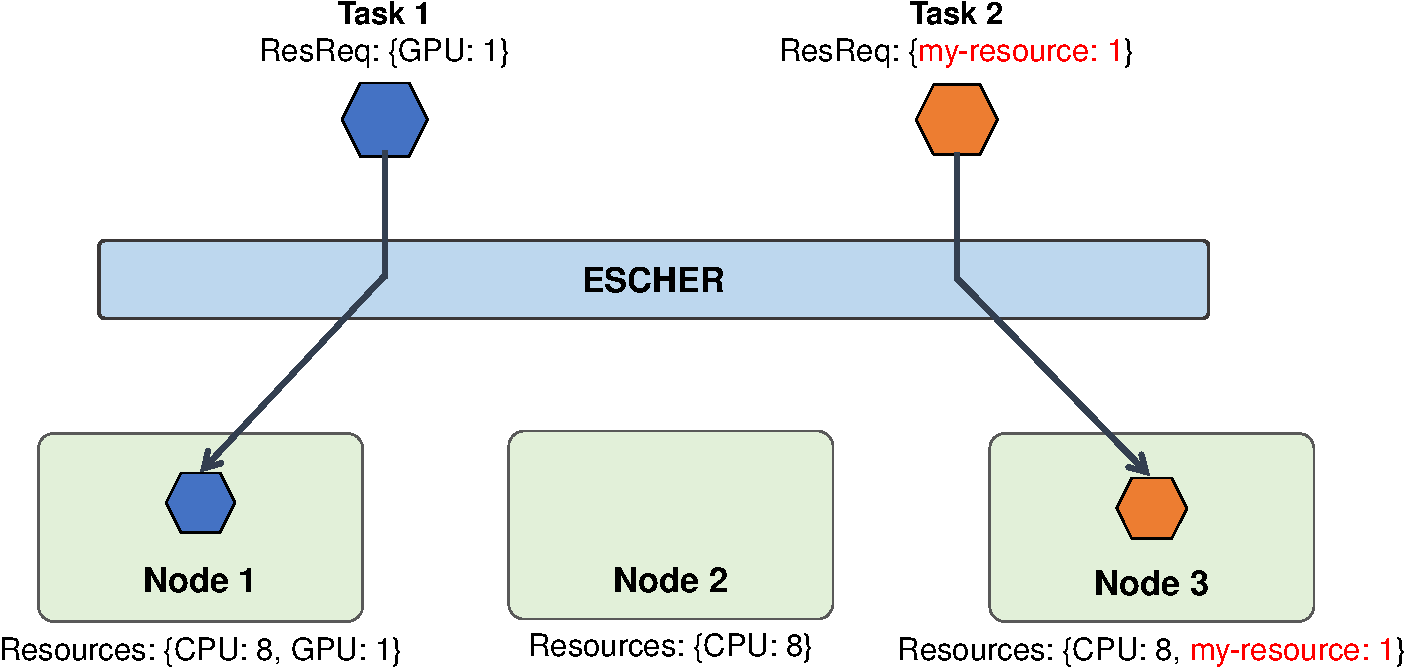
\includegraphics[width=0.82\linewidth]{escher/figures/logicalres_demo.pdf}
    \caption{Example using ephemeral resources for task placement. Applications create ephemeral resources (\emph{my-resource}) on the nodes where they wish to place a task and then launch a task requesting \emph{my-resource}. The resource-matching scheduler ensures the task is placed on the desired node.}
    %  Assuming a minimalist framework scheduler that matches task resource requests to node resource availabilities,
    \label{fig:er-example}
\end{figure}

\subsection{ESCHER workflow}
\label{sec:arch:design}

Figure~\ref{fig:esl-arch} describes the workings of an ESCHER scheduler. %, the main components of the scheduler design, and the workflow between them. 
\name{} functionality, by design, is split between the application and the resource management framework.
The application can specify scheduling policies through the ephemeral resource API (\Cref{sec:arch:api}), while the framework performs resource matching and accounting over a set of underlying physical resources.
%The framework also exposes the two ESCHER API calls, \lstinline{set_resource} and \lstinline{get_cluster_state}, to allow ephemeral resource manipulation.
We envision that most applications would specify and compose policies through the higher-level \name{} Scheduling Library~(ESL) interface, which uses the ephemeral resource API to encapsulate common policies.

%% describe a typical workflow pattern
When using ESLs, an interaction with the system typically starts with an application requesting a scheduling policy from the ESL (\cref{fig:esl-arch}).
%The ESL implements the policy by creating the appropriate ephemeral resources in the resource manager.
The ESL may interact with the resource manager, e.g., by reading cluster state, and implements the policy by creating the appropriate ephemeral resources.
The application then receives a resource specification $R$ from the ESL.
The application attaches $R$ to a task and submits it to the resource manager for placement.

\subsection{Ephemeral Resource API}
\label{sec:arch:api}

\begin{sloppypar}
In \name{}, the resource management framework exposes two simple API calls to manage ephemeral resources: \lstinline{set_resource} and \lstinline{get_cluster_status} (Listing~\ref{list:er-api}). Once created, an ephemeral resource behaves as any regular physical resource and can be acquired and released by tasks.
\end{sloppypar}

In addition to the required parameters resource label and capacity, the \lstinline{set_resource} call also allows the specification of constraints \lstinline{node_spec} where the resource must be created. If \lstinline{node_spec} is a resource vector, the resource is updated on all nodes where the constraint resource vector is a subset of the node's available resource vector.
Optionally, a \lstinline{num_nodes} field in the \lstinline{node_spec} can specify how many nodes to execute \lstinline{set_resource} on if multiple nodes satisfy the \lstinline{node_spec} constraints.
To make targeted \lstinline{set_resource} calls, the \lstinline{node_spec} can contain a unique node identifier (e.g., IP address).

The \lstinline{get_cluster_status} call returns a mapping of node to local resource capacity and availability.
These are not required for all policies, but can be useful to handle node additions and removals~(\Cref{sec:esl-faulttol}).

% \textbf{Scheduler responsibilities.}
The ESCHER scheduler's responsibility is to provide the minimal guarantees provided by any resource-matching scheduler: (1) A task whose resource requirements can be met by a node in the cluster will eventually be scheduled, and (2) A node is never allocated past its capacity.
Together, these imply that the scheduler implements: (1) task queuing and dispatch, (2) node selection for each task, and (3) resource allocation for each task.
Note that the scheduler does not need to satisfy any other constraints, such as a promise regarding the node where a task is actually scheduled.

% \swang{cut} The key difference between \name{}'s API and the APIs of existing schedulers is giving applications the ability to create and manage (ephemeral) resources at runtime. With most existing frameworks \cite{mesos,omega,yarn}, resources can be only created by operators. Also, these resources are typically created before the framework is instantiated and do not change over the lifetime of the framework. 


\begin{figure}[t]
    \centering
     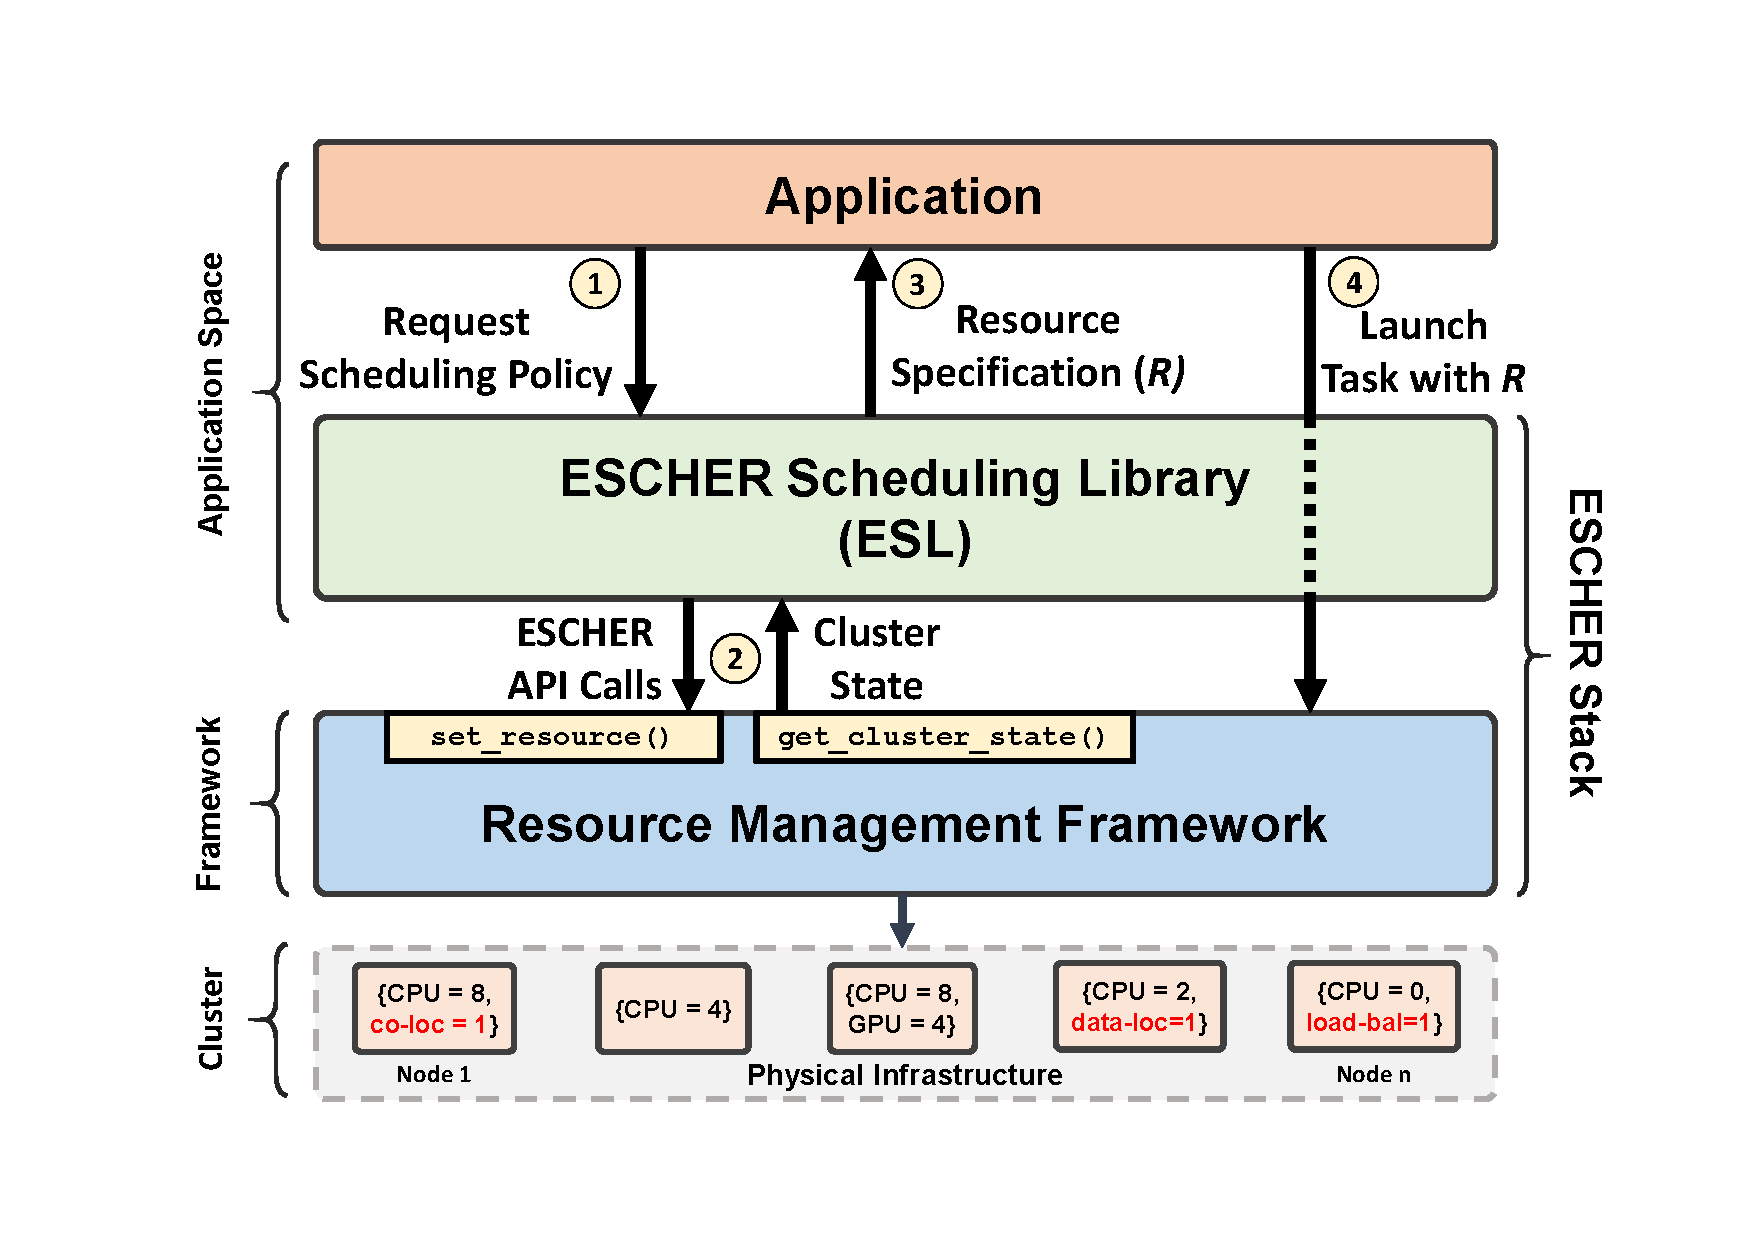
\includegraphics[width=0.85\linewidth]{escher/figures/idea_esl_arch.pdf}
    \caption{
        ESCHER task submission workflow with an ESL mediating the implementation. A task requests a supported scheduling policy from the ESL, which invokes the ESCHER API if necessary and returns the resource specification which would satisfy the policy. The task is launched with the returned resource specification.
    }
    \label{fig:esl-arch}
    \vspace{-2mm}
\end{figure}


\subsection{ESLs - \name{} Scheduling Libraries}   % Pronounced "Easel"
\label{sec:esl}

Controlling task placement through direct manipulation of ephemeral resources can be burdensome for applications with conventional scheduling requirements. 
%While the ESCHER API grants flexibility to applications to compose arbitrary scheduling policies, it requires applications to maintain ephemeral resource state and handle resource specification for tasks.
To reduce the application complexity and delineate scheduling policies from the mechanisms to implement them, we propose ESCHER Scheduling Libraries (ESLs).

The role of an ESL is simple - given a set of tasks, generate and apply a set of ephemeral resource requirements on the tasks which satisfy the desired scheduling policy.
ESLs achieve this by encapsulating the state management for ephemeral resources and providing a unified API for implementing domain-specific scheduling policies.
An application requests a scheduling policy supported by an ESL, which then makes the appropriate ESCHER API calls and returns the resource specification the application must use to realize its desired policy. In our implementations, ESLs are designed as a daemon that can service scheduling requests made from a single or multiple applications. 

ESLs are similar in spirit to Library Operating Systems (LibOS~\cite{Kaashoek:1997:APF:268998.266644}) in the Exokernel~\cite{exokernel} design.
% Just like a Library OS acts as a simplifying layer encapsulating the complexity of direct resource management exposed by an Exokernel, ESLs promote clean design and enable scheduling policies to be shared across different applications on an ESCHER scheduler.
In the same way that a LibOS encapsulates the complexity of direct resource management exposed by an Exokernel, an ESL abstracts the policy implementation and enables sharing across different applications.
% ESLs promote clean design and code re-use by abstracting all ESCHER related resource state into a unified layer that can be shared with other applications.
Moreover, this design makes applications portable across different cluster frameworks, e.g., Ray vs. Kubernetes~(\Cref{sec:impl}), since ESLs separate the application policy from the application code.
Finally, ESLs can protect applications from invalid specification of ephemeral resources by validating resource requests before launching tasks.

Since distributed applications can have widely varying scheduling requirements, we anticipate the development of domain-specific ESLs which can strike a balance between generality and preserving domain-specific optimizations. As an example, we describe and implement an ESL for hierarchical max-min fair sharing in \Cref{policies:hfs} and \Cref{eval:hfs}. % For instance, an ESL for dataframe processing applications could support data locality and task co-location, while adding implicit data replication at the ESL layer to improve data locality. As an example, we describe and implement an ESL for hierarchical max-min fair sharing in \cref{policies:hfs} and \cref{eval:hfs}.

% \subsubsection{\romilc{Example ESL - Ray Placement Groups}}
% % How can I use ESLs? You can do affinity plus gangn scheduling with ESLs. Show how they can compose. 
% \romilc{Ray\cite{ray} utilizes ephemeral resources to implement a ESL called the placement groups API. Placement groups allow users to atomically reserve groups of resources across multiple nodes (i.e., gang scheduling). They can be then used to schedule Ray tasks and actors to be packed as close as possible for locality (PACK qualifier), or spread apart (SPREAD qualifier).}

% \romilc{Ray placement groups operate by creating bundles of resources which can be atomically reserved by tasks. These bundles are reserved by creating ephemeral resources which replace the physical resources with unique virtual instances which are unique to a specific task. In other words, once a placement group is created, the original physical resources are consumed by the placement group, and ephemeral resources are then consumed by the task. The ESL manages the lifecycle of these ephemeral resources by creating them when tasks request a placement group and releasing them when the task ends.}

% \romilc{\romil{Fault tolerance?}If nodes that contain some bundles of a placement group die, all the bundles will be rescheduled on different nodes by Ray using the ephemeral resource API. This means that the initial creation of placement group is “atomic”, but once it is created, there could be partial placement groups.}


\begin{listing}
\begin{minted}{python}
# Create resource with name and capacity on a node 
# where the 'node_spec' constraints are satisfied.
# node_spec can be a resource vector or node id.
# If node_spec = None, resource is set locally
def set_resource(name, capacity, node_spec)

# Returns cluster resource state as a list of 
# node-wise map of local resource availability.
def get_cluster_status()
\end{minted}
\caption{Ephemeral resource API}
\vspace{-1em}
\label{list:er-api}
\end{listing}

\subsection{Fault tolerance}
\label{sec:esl-faulttol}
In the event of a node failure, ESCHER works in tandem with the fault-tolerance scheme of the underlying framework. Most frameworks~\cite{ray,kubernetes} simply re-execute the tasks with the same resource requirement. However, since these resource requests include ephemeral resources which no longer exist, these re-executed tasks cannot be scheduled.

At the bare minimum, an ESL must ensure that ephemeral resources are restored at some other eligible node. To do this, ESCHER relies on the cluster framework to report failed nodes through the \lstinline{get_cluster_status} API. Once failed nodes are detected, an ESL can recreate the ephemeral resources on suitable nodes by replaying the \lstinline{set_resource} calls for the failed resources. If a candidate node is found, the resource is recreated, else the tasks must wait for the failed node to recover before they can be rescheduled. When a node is restored, its resources are also reinitialized, allowing any waiting tasks to get rescheduled. % In addition to this basic policy, ESLs can define application-specific recovery routines.% after the ephemeral resources are restored.

\subsection{Evolvability and complexity in \name{}}
\label{sec:arch:evolve}
The ability to create ephemeral resources on targeted nodes makes scheduling with ESCHER as flexible as letting the application directly
control task placement on cluster nodes. %schedule its tasks on any node in the cluster. 
Indeed, scheduling a task $T$ on node $N$ is equivalent to assigning a uniquely-named ephemeral resource $R_N$ with capacity 1 to node $N$, and having $T$ request one unit of resource $R_N$. 


% Should this go in related work
While this targeted placement makes ESCHER highly evolvable, what are its benefits over simply
yielding placement control over resources to the application directly?
% giving the application direct access to the cluster's resources? 
After all, if the goal is to schedule a task on a particular node, ESCHER makes this operation arguably more complex as it requires creating an ephemeral resource on the node.% to place the task there.

The primary benefit of ESCHER is that policy and ESL implementations do not need to reason about \emph{tasks}.
In a framework with fully application-level scheduling, such as Mesos or Omega \cite{mesos, omega}, the application scheduler has to maintain possibly distributed state about the current set of tasks.
When a task is submitted and can't yet be scheduled, the scheduler queues the task.
When a task starts, the scheduler must update the current resource availability to ensure that resources do not become oversubscribed.
On task completion, the scheduler must again update the current resource availability and select a new task to run from the queue.

Of course, none of these functionalities are unique to ESCHER.
Task to resource matching is a necessity to every scheduler system, which is why it is the core responsibility that we assign to the ESCHER scheduler.
Thus, in ESCHER, \emph{an application that has no specific policy requirements can use an ESCHER scheduler directly without implementing any scheduling code}.
This is not possible in systems that expose resources directly to the application, such as Mesos~\cite{mesos} or Omega~\cite{omega}, as it is expected that the application will also implement all mechanisms related to task scheduling.

For applications that do require a custom policy or an ESL, this division of responsibilities still reduces the effort required from the application developer, compared to implementing a complete scheduler.
For example, most of the policies that we present in \Cref{tab:escher-constraints-policies} do not require examining the current cluster state; it is enough for a task to create a resource on its local node or create resources on all nodes that match a given resource spec.
The exceptions are gang scheduling, which requires reading the cluster state to roll back a group of tasks in case of a failure, and load-balancing, which computes the current load from the cluster state.
In contrast, a fully application-level scheduler must continually update and reason about the current cluster state in order to find a suitable node for each task.
In the ESCHER design, this responsibility is given to the system rather than the application.
%\camready{ESLs don’t concern themselves with physical resource allocation, only consumption and creation of ephemeral resources.}

% ESCHER provides three key benefits over exposing the cluster’s resources to the application.
% %and letting the application implement scheduling policies from scratch. 
% \textbf{[R1]} First, it offers a single source of the global resource availability truth. %of the nodes across the cluster. 
% In the absence of this mechanism, it's up to each individual application to do so. This is problematic for many reasons.
% Local application's view of resources must be maintained on start/completion of each resource consuming task and each resource-bearing node arrival/departure. This requires each application to be fault-aware.
% % If we just expose the cluster’s resources to the application, the application needs to keep track of the cluster’s resource availability itself. In particular, when a task starts or finishes, the application needs to update the node’s resource availability. Furthermore, the application needs to update this availability as nodes fail, which means it needs to detect failures. 

% \textbf{[R2]} Second, distributed application resource state tracking/management can easily lead to resource coordination failures  potentially causing deadlocks. When multiple applications maintain their local view of the same shared resource availability state, maintaining consistency of this state in a distributed system is a complex problem, especially in the presence of node and task failures. This requires implementation of expensive distributed consensus protocols or optimistic concurrency mechanisms (e.g., Omega~\cite{omega}). Surprisingly, even with proper distributed resource state management, applications may still enter livelock situations when they incrementally request resources to satisfy complex constraints, such as gang scheduling constraints (e.g., Mesos~\cite{mesos}).
% % Finally, if there are multiple applications sharing the same cluster they have to somehow share the availability state. This is a complex problem as it reduces to maintaining the consistency of the state (i.e., node resource availability) in a distributed system in the presence of failures. 

% \textbf{[R3]} Third, ephemeral resources enable applications to naturally express an exhaustive family of scheduling constraints. 
% We consider scheduling constraints of three types: 
% (a) \textbf{spatial}: a \textit{where} constraint on resource properties required for task placement (e.g., GPUs, CPU architecture, memory, availability of executable binaries~\cite{bikash-google-socc11});
% (b) \textbf{temporal}: a \textit{when} constraint on the relative ordering of tasks with respect to each other. Examples include gang scheduling (temporally simultaneous). 
% (c) \textbf{task-task}: constraints irrespective of the physical properties of underlying resources or time. These include constraints or preferences on the virtual task topology, e.g., Scheduling a directed acyclic graph (DAG) of tasks.
% %with clusters of tasks exhibiting structural coupling within tasks in each cluster and loose coupling across the clusters. Scheduling a directed acyclic graph (DAG) of tasks is another distinct class of task-task constraints. 
% The ``happens-before'' relationship between tasks is notoriously difficult to express declaratively (e.g., not supported by state-of-the-art DCM~\cite{dcm-osdi20} and TetriSched~\cite{tetrisched}) and requires specialized imperative heuristics, sacrificing both evolvability and generality (e.g., Spark DAG Scheduler~\cite{spark-dagscheduler}).
% Fundamentally, ESCHER's dynamic ephemeral resources serve as a \textit{reduction mechanism}, reducing both, task-task constraints to spatial or temporal, and temporal constraints to spatial. We exemplify this novel reduction mechanism in Table~\ref{tab:escher-constraints-policies}.

% define \textit{a scheduling constraint} as a constraint on resource properties required for task placement (spatial) or a constraint on the ordering of tasks relative to each other (temporal). Examples incl
% By \textit{scheduling constraints} we mean any constraint imposed on scheduling two or more tasks, such as running two tasks at the same time (i.e., gang scheduling), co-locating two tasks (i.e., affinity) and co-locating data with computation (i.e., locality-aware scheduling). In particular, \name{} enables applications to cast scheduling constraints as ephemeral resource constraints, and then lets its resource-constrained scheduler enforce these constraints. For example, to implement locality-aware scheduling, an application can assign to each data item a uniquely-named ephemeral resource and then add the ephemeral resource associated with a task’s input to its resource requirements. \name{} does the rest. If a data item is replicated on multiple nodes, this solution works without any changes; just assign the same ephemeral resource to every node storing a replica of the data item. In contrast, if we just expose the cluster resources to the application, the application will need to keep track of the mapping between data items and nodes storing these data items, which again reduces to maintaining the state consistent in a distributed system.